\documentclass[border=3pt]{standalone}
% Preâmbulo compartilhado pelos diagramas TikZ da aula 6 de IHC (Necessidades e Requisitos)
\usepackage[T1]{fontenc}
\usepackage[utf8]{inputenc}
\usepackage{lmodern}
\usepackage{amsmath}
\usepackage{xcolor}
\usepackage{tikz}
\usetikzlibrary{arrows.meta,angles,quotes,decorations.pathmorphing,calc,
                positioning,shapes.geometric,shapes.misc,backgrounds,fit,
                math}

% Paleta (mesma dos SVGs originais)
% Paleta da disciplina de IHC: acento roxo (#755099), da capa do livro.
% (o nome "dblue" é mantido para não alterar todos os diagramas)
\definecolor{dblue}{HTML}{755099}
\definecolor{dorange}{HTML}{B3541E}
\definecolor{dgreen}{HTML}{4A7C59}
\definecolor{dred}{HTML}{9C4B4B}
\definecolor{dcream}{HTML}{F4F1EA}
\definecolor{dshade}{HTML}{DDD7C9}

% Função gaussiana (não normalizada por padrão de escala visual)
\pgfmathdeclarefunction{gauss}{3}{%
  \pgfmathparse{1/(#3*sqrt(2*pi))*exp(-((#1-#2)^2)/(2*#3^2))}%
}

% Estilos comuns (prefixo d... para não colidir com chaves internas do pgf)
\tikzset{
  >={Stealth[length=2mm]},
  dguide/.style={gray!55, dashed, line width=0.4pt},
  daxis/.style={gray!60, line width=0.7pt, ->},
  dbody/.style={fill=black!3, draw=black!80, line width=1pt},
  dacc/.style={draw=dblue, line width=1pt},
  dlbl/.style={black!55, font=\small},
  dsub/.style={black!45, font=\footnotesize},
  dstate/.style={circle, draw=black!80, fill=dcream, line width=1pt,
                 minimum size=17mm, font=\large, inner sep=1pt},
  dobs/.style={circle, draw=black!80, fill=dshade, line width=1pt,
               minimum size=14mm, font=\large, inner sep=1pt},
  dbox/.style={rounded corners=2pt, draw=black!80, fill=dcream, line width=1pt,
               align=center, inner sep=6pt},
  dop/.style={circle, draw=black!80, fill=white, line width=1pt,
              minimum size=6mm, inner sep=0pt, font=\small},
  dtrans/.style={->, dblue, line width=1pt},
  dmeas/.style={->, dorange, line width=1pt},
  dcurve/.style={line width=1pt, dblue},
  dcurveb/.style={line width=1.4pt, dorange},
}

\begin{document}
\hyphenpenalty=10000 \exhyphenpenalty=10000 \tolerance=9999 \emergencystretch=3em
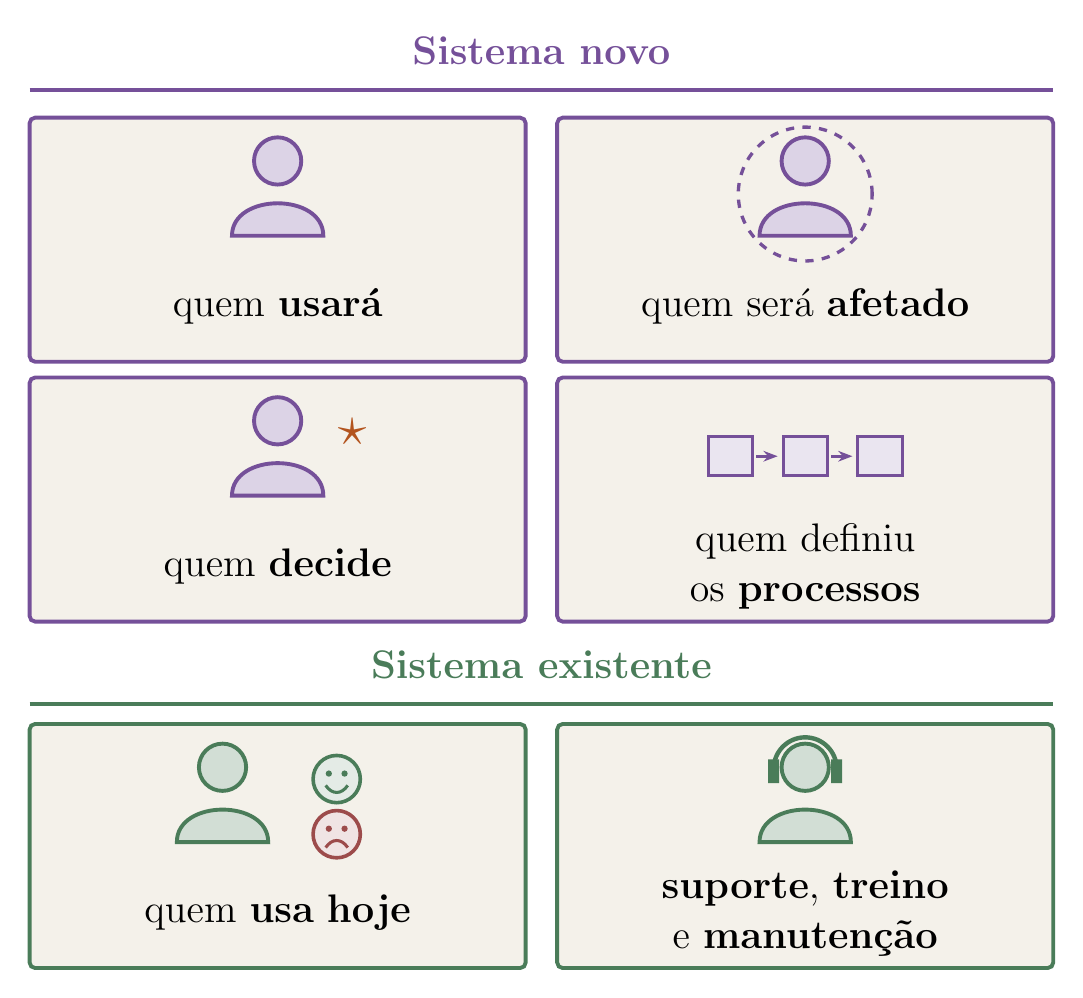
\begin{tikzpicture}[x=1cm,y=1cm]
\node[font=\Large\bfseries, dblue] at (6.50,12.00) {Sistema novo};
\draw[dblue, line width=1.4pt] (0,11.50) -- (13.00,11.50);
\node[dbox, draw=dblue, line width=1.4pt, minimum width=6.3cm, minimum height=3.1cm] at (3.15,9.60) {};
\fill[dblue!25!white, draw=dblue, line width=1.4pt] (3.15,10.60) circle (0.3);
\fill[dblue!25!white, draw=dblue, line width=1.4pt] (2.57,9.65) .. controls (2.57,10.20) and (3.73,10.20) .. (3.73,9.65) -- cycle;
\node[font=\Large, text width=5.7cm, align=center] at (3.15,8.75) {quem \textbf{usará}};
\node[dbox, draw=dblue, line width=1.4pt, minimum width=6.3cm, minimum height=3.1cm] at (9.85,9.60) {};
\draw[dblue, dashed, line width=1.2pt] (9.85,10.18) circle (0.85);
\fill[dblue!25!white, draw=dblue, line width=1.4pt] (9.85,10.60) circle (0.3);
\fill[dblue!25!white, draw=dblue, line width=1.4pt] (9.27,9.65) .. controls (9.27,10.20) and (10.43,10.20) .. (10.43,9.65) -- cycle;
\node[font=\Large, text width=5.7cm, align=center] at (9.85,8.75) {quem será \textbf{afetado}};
\node[dbox, draw=dblue, line width=1.4pt, minimum width=6.3cm, minimum height=3.1cm] at (3.15,6.30) {};
\fill[dblue!25!white, draw=dblue, line width=1.4pt] (3.15,7.30) circle (0.3);
\fill[dblue!25!white, draw=dblue, line width=1.4pt] (2.57,6.35) .. controls (2.57,6.90) and (3.73,6.90) .. (3.73,6.35) -- cycle;
\node[font=\huge, dorange] at (4.10,7.15) {$\star$};
\node[font=\Large, text width=5.7cm, align=center] at (3.15,5.45) {quem \textbf{decide}};
\node[dbox, draw=dblue, line width=1.4pt, minimum width=6.3cm, minimum height=3.1cm] at (9.85,6.30) {};
\draw[dblue, fill=dblue!15!white, line width=1.1pt] (8.62,6.60) rectangle ++(0.56,0.5);
\draw[dblue, fill=dblue!15!white, line width=1.1pt] (9.57,6.60) rectangle ++(0.56,0.5);
\draw[dblue, fill=dblue!15!white, line width=1.1pt] (10.52,6.60) rectangle ++(0.56,0.5);
\draw[dblue, -{Stealth[length=1.8mm]}, line width=1.1pt] (9.23,6.85) -- (9.50,6.85);
\draw[dblue, -{Stealth[length=1.8mm]}, line width=1.1pt] (10.18,6.85) -- (10.45,6.85);
\node[font=\Large, text width=5.7cm, align=center] at (9.85,5.45) {quem definiu os \textbf{processos}};
\node[font=\Large\bfseries, dgreen] at (6.50,4.20) {Sistema existente};
\draw[dgreen, line width=1.4pt] (0,3.70) -- (13.00,3.70);
\node[dbox, draw=dgreen, line width=1.4pt, minimum width=6.3cm, minimum height=3.1cm] at (3.15,1.90) {};
\fill[dgreen!25!white, draw=dgreen, line width=1.4pt] (2.45,2.90) circle (0.3);
\fill[dgreen!25!white, draw=dgreen, line width=1.4pt] (1.87,1.95) .. controls (1.87,2.50) and (3.03,2.50) .. (3.03,1.95) -- cycle;
\draw[dgreen, line width=1.3pt, fill=dgreen!15!white] (3.90,2.75) circle (0.3);
\fill[dgreen] (3.80,2.82) circle (0.04) (4.00,2.82) circle (0.04);
\draw[dgreen, line width=1.1pt] (3.76,2.67) .. controls (3.84,2.55) and (3.96,2.55) .. (4.04,2.67);
\draw[dred, line width=1.3pt, fill=dred!15!white] (3.90,2.05) circle (0.3);
\fill[dred] (3.80,2.12) circle (0.04) (4.00,2.12) circle (0.04);
\draw[dred, line width=1.1pt] (3.76,1.88) .. controls (3.84,2.00) and (3.96,2.00) .. (4.04,1.88);
\node[font=\Large, text width=5.7cm, align=center] at (3.15,1.05) {quem \textbf{usa hoje}};
\node[dbox, draw=dgreen, line width=1.4pt, minimum width=6.3cm, minimum height=3.1cm] at (9.85,1.90) {};
\fill[dgreen!25!white, draw=dgreen, line width=1.4pt] (9.85,2.90) circle (0.3);
\fill[dgreen!25!white, draw=dgreen, line width=1.4pt] (9.27,1.95) .. controls (9.27,2.50) and (10.43,2.50) .. (10.43,1.95) -- cycle;
\draw[dgreen, line width=1.6pt] (9.45,2.88) arc (180:0:0.4);
\fill[dgreen] (9.38,2.70) rectangle ++(0.14,0.3) (10.18,2.70) rectangle ++(0.14,0.3);
\node[font=\Large, text width=5.7cm, align=center] at (9.85,1.05) {\textbf{suporte}, \textbf{treino} e \textbf{manutenção}};
\end{tikzpicture}
\end{document}
